\documentclass[main.tex]{subfiles}

\begin{document}
    \chapter[Formation of Compact Twin Stars in Low-Mass X-Ray Binaries]{Formation of Compact Twin Stars in Low-Mass X-Ray Binaries}
    % \chaptermark{Astrophysical Consequences of Dense Matter Phase Transitions}


    \begin{center}
        \textbf{S. Chanlaridis}, D. Ohse, D. E. Alvarez-Castillo, J. Antoniadis, D. Blaschke, V. Danchev, N. Langer, and D. Misra   \\

        \vspace{0.5cm}

        Accepted for publication in Astronomy \& Astrophysics
    \end{center}
        
        
    \begin{center}
        \textbf{\large Abstract}
    \end{center}
    
    {\hypersetup{linkcolor=black, pdfborder={0 0 0}}
        \minitoc
        \newpage
    }
    
    \section{Introduction} \label{sec:intro}
        Millisecond pulsars (MSPs) are widely considered to be old, spun-up neutron stars (NSs) characterized by high rotational frequencies, $\mathcal{O}(10^2\,\rm Hz)$, and weak surface magnetic fields, $\mathcal{O}(10^8\,\rm G)$. The formation of MSPs can be traced back to a recycling
        phase in a low-mass X-ray binary \citep[LMXB; see][]{Tauris:2023nmj}. 
        During the recycling process,  mass and angular momentum are accreted onto the NS from the companion star when the latter fills its Roche lobe \citep[e.g.,][and references therein]{Bhattacharya:1991pre, Tauris:aap1999, Tauris:2023nmj}. During mass transfer,, tidal interactions circularize the orbit on a timescale that is much shorter $(\sim 10^4\,\rm yr)$ than the  mass accretion phase. Therefore, MSPs are expected to populate binary systems with very small eccentricities \citep{Phinney:1992, Verbunt:aa1995}.
        
        Although the vast majority of MSPs are indeed situated in systems with highly circularized orbits, a considerable fraction  appear to be solitary \citep[$\sim 27$\% among known MSPs with spin periods $\leq 30$\,ms; see the ATNF pulsar catalogue;][]{Manchester_2005}\footnote{\url{https://www.atnf.csiro.au/research/pulsar/psrcat/}\\ accessed on 29 May 2024}. These isolated MSPs (iMSPs) raise questions about the recycling process, particularly about possible mechanisms that could eject, consume, or disrupt the MSP companion stars \citep{1987Natur.329..312V, 2019PASA...36....5S, 2019JApA...40...32N, 2020A&A...633A..45J}. 
        
        
        In addition, recent pulsar surveys have revealed the existence of binary MSPs with eccentricities of up to $e \simeq 1$. With
        the exception of MSPs in globular clusters, and PSR\,J1903+0327 \citep{Champion:sci2008} which is a Galactic field MSP with a
        main-sequence companion and an eccentricity of $e\simeq0.9$, 
         eccentric MSPs (eMSPs) appear to have orbital periods between 20 and 50\,d, and eccentricities $\mathcal{O}(0.1)$, 
         \citep{Deneva:apj2013, Barr:mnras2013, Knispel:apj2015, Camilo:apj2015, Octau:aap2018, Stovall:apj2019}. 
        Although chaotic gravitational interactions, such as the ejection of the least massive member of a hierarchical triple system
        progenitor, have the potential to explain the formation of eMSPs in clusters \citep[e.g.,][]{2011MNRAS.412.2763F, 
        2011ApJ...734...55P},   they are unlikely to produce systems that have similar binary parameters \citep[see][]
        {Deneva:apj2013, Barr:mnras2013, Knispel:apj2015, Camilo:apj2015, Octau:aap2018}, such as those found in the Galactic field. 
        However, several attempts have been made to investigate alternative formation channels that can accommodate the observed properties of eMSPs \citep[e.g., see ][for an overivew of various eMSP formation scenarios]{Freire:mnras14, antoniadis:apjl14, Jiang:apj15, Jiang:raa2021, ginzburg:mnras21}. 
        
        One possible way to explain the formation of both iMSPs and eMSPs might be related to abrupt changes in the interior of the NS
        \citep{Freire:mnras14, Jiang:apj15, Alvarez-Castillo:2019apz}. For instance, the dependence of the NS structure on the
        equation of state (EoS) highlights the possibility of exotic phases and phase transitions in their interiors. An interesting
        scenario is the existence of a third family of compact stars \citep[see][]{Gerlach:1968zz}
        beyond the conventional  white dwarf (WD) and NS classifications. 
        Such a third family could emerge as a result of a phase transition in the NS core, leading to the formation of
        hybrid stars with an outer core of hadronic matter and an inner core of deconfined quark matter \citep[e.g.,][]
        {Schertler:2000xq,Benic:2014jia, Alvarez-Castillo:2019apz, 2021AN....342..234A}. 
        
        Within the context of MSP formation scenarios, such an instantaneous transition to the third family branch could be
        triggered during, or after, the LMXB phase due to mass accretion from the donor star \citep[see, e.g.,][]
        {Bejger:2016emu,Alvarez-Castillo:2019apz}. This transition could, in turn, induce instantaneous mass loss and/or a kick  that can cause significant changes to the orbital dynamics \citep{Jiang:apj15}. 
        More specifically, the sudden decrease in gravitational mass due to quark deconfinement in the core \citep[owing to the ``catastrophic rearrangement'' and strong compactification of matter when transitioning to the third-family branch which increases the gravitational binding energy, see ][]{Mishustin:2002xe}, may significantly increase eccentricity or even disrupt the binary \citep[see also][]{Jiang:raa2021}. The main aim of this work is to explore this possibility in more detail. 
        
        The investigation of such scenarios is important for advancing our understanding of dense matter under extreme conditions.  Recent advances in observational techniques, such as gravitational wave detections from NS mergers and high-precision pulsar timing, offer unprecedented opportunities to test and refine such theoretical models predicting phase transitions \citep[e.g.,][]{PhysRevLett.119.161101}.
        For instance, gravitational waves from unstable fundamental $f$-mode oscillations can reveal the internal stellar
        structure and matter distribution characteristic of a first-order phase transition, as shown in \cite{2023arXiv230908775K} 
        where the estimations for the same class of models used in this work are presented, or in \cite{2023arXiv231115992K} where
        accretion into compact stars is considered, resulting in the same mechanism of production of gravitational radiation from
        $f$-mode excitation and the associated neutrino emission. It is indeed expected that with the precision of the next generation of gravitational wave detectors, these scenarios can be studied. 
        All in all, the timely synergy between theoretical developments and observational capabilities places us at the forefront of uncovering the complex NS physics, where phase transitions emerge as a central theme \citep{Bauswein:2022vtq}.
        
        
        In this work, we combine detailed binary evolution calculations with a simple analytic model for the response of the NS spin and radius to accretion to investigate whether first-order phase transitions could lead to the formation of eMSPS and iMSPs. The text is organized as follows: In Sect.~\ref{sec:methods} we describe the methodology and physical assumptions. We present the results of our simulations in Sect.~\ref{sec:results} and in Sect.~\ref{sec:uncertainties} we discuss various uncertainties related to them. We conclude with a summary and a discussion on the implications of our calculations in Sect.~\ref{sec:summary}.
            

    \section{Methodolody} \label{sec:methods}
    
    \subsection{Initial setup and numerical calculations}\label{sec:setup}
    
        Our main goal is to investigate first-order phase transitions in accreting MSPs using stellar evolution calculations. To this end, our working setup is divided into three distinct components:
        
        \begin{enumerate}
            \item An EoS for dense nuclear matter that allows for a first-order phase transition. 
            \item A stellar evolution model for the binary system, providing the mass-accretion profile as a function of time for the NS. 
            \item An accretion model that allows us to calculate the spin, mass, and radius evolution of the NS during and after the LMXB phase.
        \end{enumerate}
        These are described in detail in the remainder of the section.
        
        \subsubsection{Equation of state and mass-radius relation}\label{sec:eos}
        For the EoS, we select a multipolytrope model suitable for describing both nuclear and quark matter within NSs. This EoS is chosen for its ability to: (a) account for a strong first-order phase transition from hadronic to quark matter above $1.4\msun$ (depending on the angular momentum) and (b) satisfy current constraints derived from multimessenger astronomy \citep{antoniadis:2013sci, LIGOScientific:2018cki, 2019ApJ...887L..21R, 2019ApJ...887L..24M, 2020NatAs...4...72C}.
        
        The outer layers, characterized by densities $n \leq 0.5 n_0$, where $n_0$ denotes the nuclear saturation density, are modeled using the \texttt{BPS} EoS \citep{Baym:1971apj}. An intermediate density regime with $0.5 n_0 < n \leq 1.1 n_0$ is assumed to consist of homogeneous matter in $\beta$-equilibrium. For regions with densities $n > 1.1 n_0$ we distinguish four regimes, each one of them described by a polytropic equation of state of the form:
        
        \begin{equation}
            P(n) = \kappa_i \left( \frac{n}{n_0} \right)^{\Gamma_i},
            \label{eq:acb5_eos}
        \end{equation}
        henceforth referred to as the \texttt{ACB5} EoS as in \cite{Paschalidis:2018prd}.
        
        The first polytrope, $(i=1)$, is a fit to the stiffest EoS version provided in \cite{Hebeler:2013apj}. The second polytrope, $(i=2)$, describes the first-order phase transition. The polytropic index $\Gamma$ allows us to distinguish between a sharp transition (Maxwell construction, $\Gamma = 0$) and a non-sharp transition (Gibbs construction, $\Gamma \neq 0$). Since we require a strong transition to produce a large jump in energy density, the second polytrope is defined as a region of constant pressure $P_c = \kappa_2$, where $\Gamma_2 = 0$ is imposed by the Maxwell construction. The remaining two polytropes $(i = 3,4)$ describe regions with densities that exceed the critical value for a first-order transition and correspond to stiff quark matter which should be able to support a NS with masses up to $\sim 2.0\msun$ \citep[e.g.,][]{2020NatAs...4...72C}.
        The different density regimes are thermodynamically joined in a consistent manner. 
        
        To infer the corresponding mass-radius relation for rigidly spinning NSs, we used the numerical integrator described in \cite{Alvarez-Castillo:2019apz}. 
        In this code, the integration of the structure equations proceeds radially outward from the center of the NS, where the density is highest, to its surface, where the pressure falls to zero, thus determining the total mass and radius for various central densities and angular momenta, $J$. 
        
        The resulting mass-radius relations are illustrated in Fig.~\ref{fig:mvsr}. 
        The lower right section of the figure, depicts the mass-radius relation for NSs within the hadronic branch, corresponding to the \texttt{ACB5} first polytrope and indicating a composition of purely hadronic matter. Moving towards the upper left segment of the figure, we shift into the hybrid star branch, representing NSs that have undergone a phase transition to include a quark matter core, described by the \texttt{ACB5}'s third and fourth polytropes. This transition is shown by a dashed black curve, representing the second polytrope of the \texttt{ACB5} EoS and indicating the hadronic branch's point of maximum stability---that is, the highest mass that a NS composed entirely of hadronic matter can sustain. Beyond this threshold, additional mass triggers a phase transition to quark matter, moving the star to the hybrid branch.
        
        The role of spin and angular momentum in dictating the precise moment of transition is crucial; higher angular momentum allows a NS to support more mass in the hadronic phase. This effect is illustrated by the 
        different colors, which denote varying levels of angular momentum, normalized by $J_0 = \displaystyle GM_\odot^2/c$. Here, the solid black line represents a static NS, and the outermost (light-yellow) line corresponds to $J/J_0 = 0.45$. Beyond this point, the hadronic branch extends past the shedding limit, where equatorial matter attains Keplerian escape velocity and is ejected.
        
        For the calculations that follow, we assume that a NS reaching the transition line undergoes a phase transition on the dynamic timescale, under conservation of the angular momentum and baryonic mass. 
        The transition moves the NS from the maximal stability threshold on the hadronic branch (dashed line), to a corresponding position (in terms of angular momentum and baryonic mass) on the third family. This principle is visually represented by the magenta curve linking points on the hybrid branch that could be attained through the transition and defining the birth mass of the twin star. 
        
        
        \begin{figure}
            \centering
            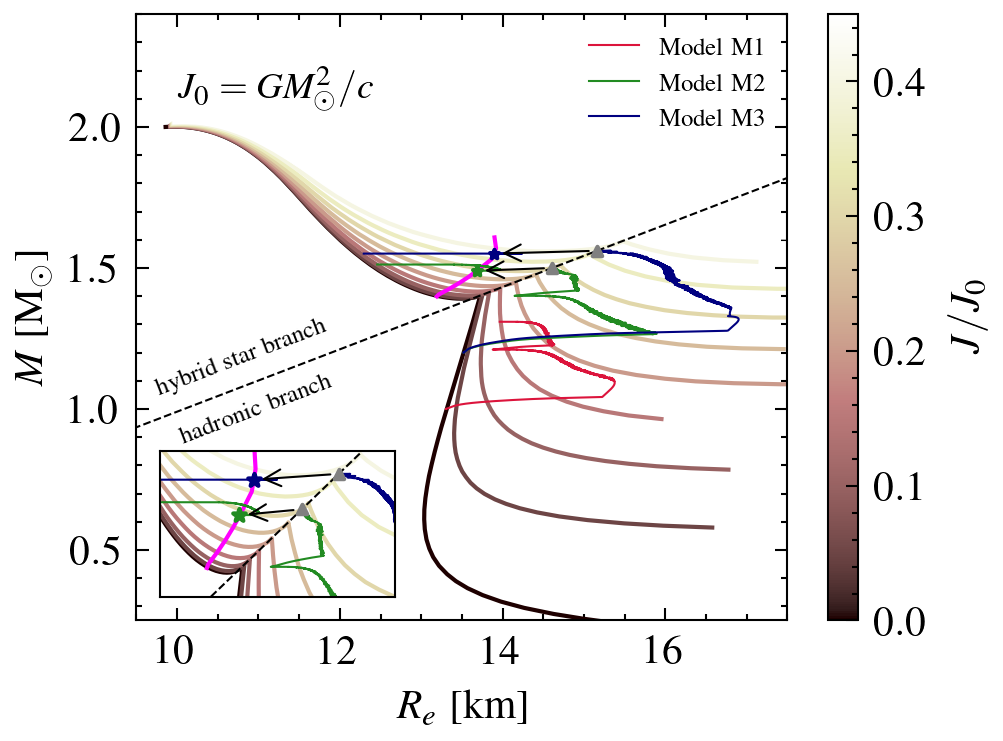
\includegraphics[width=0.5\columnwidth]{figures/chapter3/m_vs_r.png}
            \caption{Gravitational mass versus equatorial radius for our \textsc{m1} (red), \textsc{m2} (green), and \textsc{m3} (blue) binary models. The magenta curve connects those points on the hybrid star branches which can be reached by a collapse from the maximum of stability on the hadronic branch under conservation of angular momentum, $J$, and baryonic mass $M_b$. The star marks indicate the trajectory endpoint for the direct (\textsc{m2}) and delayed collapse (\textsc{m3}) models. Note the arrows are inclined, since the ordinate is gravitational mass and not baryonic mass.}
            \label{fig:mvsr}
        \end{figure}
        
    
    
    \subsubsection{Mass transfer and binary evolution models} \label{sec:input_params}
        To obtain realistic mass transfer models, we performed detailed numerical binary calculations using the implicit one-dimensional code \textbf{M}odules for \textbf{E}xperiments in \textbf{S}tellar \textbf{A}strophysics \citep[\mesa\,v12778;][]{Paxton:2010ji,Paxton:2013pj,Paxton:2015jva,Paxton:2017eie}. Our binary systems consist of a zero-age main sequence (ZAMS) donor and a NS accretor, which is treated as a point mass.
        We calculated three models chosen as representative of three distinct cases: a LMXB in which a phase transition never occurs (model \textsc{m1}), one in which the transition occurs during the mass transfer phase (\textsc{m2}), and a model for which the transition occurs after the accretion phase, due to the NS spin down (\textsc{m3}). The initial binary parameters for each model are summarized in Table~\ref{tab:config}.
        
        \begin{table}[t]
            \centering
            \caption{Initial binary parameters for our stellar evolution models.}
            \begin{tabular}{cccc}
                 \hline \hline \\
                 Model & $M_\mathrm{don}\,[\msun]$ & $M_\mathrm{ns}\,[\msun]$ & $P_\mathrm{orb}\,[\mathrm{days}]$  \\
                 \hline \\
                \textsc{m1} & $1.0$ & $1.0$ & $8$ \\\\
                \textsc{m2} & $1.0$ & $1.2$ & $8$ \\\\
                \textsc{m3} & $1.0$ & $1.2$ & $22.627$ \\\\
                \hline
            \end{tabular}
            \label{tab:config}
        \end{table}
        
        Convection was modeled using the modified mixing length theory (MLT) prescription of \cite{Henyey:apj1965} with a mixing-length parameter of $\alpha_{\rm ML} = 1.8$. In our models, we enable convective premixing while trying to avoid increases in the abundance of species that are burnt, where  possible. Stability against convection was determined according to the Ledoux criterion \citep[][]{Ledoux:apj1947}. Additionally, we employed semi-convection, which we treated as a diffusive process, with an efficiency parameter of $\alpha_{\rm SEM} = 1.0$ \citep[][]{Langer:aap1991}. Lastly, we account for the overshooting of convective material beyond the convective layers by adopting an exponential overshooting efficiency of $f_{\rm ov, core} = 0.016$ and $f_{\rm ov, env} = 0.0174$ in the core and envelope, respectively. 
        
        Rotational mixing was taken into consideration, including the effects of Eddington–Sweet circulations, secular and dynamical instability, and the Goldreich–Schubert–Fricke instability \citep[see][for details]{Heger:apj2000}. The contribution of these instabilities to the total diffusion coefficient was reduced by a mixing efficiency factor, $f_c = 1/30$ \citep[][]{1992A&A...253..173C, Heger:apj2000}. Moreover, we employed the Spruit-Tayler dynamo to compute the internal magnetic field strength and the corresponding transport of angular momentum, as described in \cite[][]{Spruit:aap2002, Heger:apj2005}.
        
        To calculate the mass loss rate due to stellar wind that the donor stars experience during their evolution, we implemented the cool red giant branch wind scheme by \cite{Reimers:bk1975}:
        \begin{equation}
            \label{eq:reimers_mdot}
            \dot{M}_{1, \text{wind}} = -4 \times 10^{-13} \eta \left(\frac{R_1}{R_\odot}\right) \left(\frac{L_1}{L_\odot}\right)\left(\frac{M_\odot}{M_1}\right)\quad [M_\odot\,\text{yr}^{-1}],
        \end{equation}
        using a scaling factor of $\eta = 0.1$. In cases of hydrogen-poor donor stars, where their hydrogen mantle has been stripped (surface hydrogen mass fraction $X_{\rm S} < 0.4$), we applied the prescription of \cite{Nugis:aap2000} for Wolf-Rayet stars with a scaling factor of $\eta = 1.0$. The latter is used in \mesa under the \texttt{Dutch} hot wind scheme \citep[][]{Glebbeek:aap2009}. 
        
        We assumed that our binary models are initially tidally synchronized to the orbit at the beginning of the evolution (ZAMS stage) and that the eccentricity is negligible. These assumptions are justified as tidal forces would circularize (and synchronize) the orbit on a much shorter timescale compared to the main-sequence lifetime of a low-mass donor star \citep[e.g.,][]{Verbunt:aa1995}.
        
        To compute the mass transfer rates during Roche-lobe overflow (RLOF) we used the prescription suggested by \cite{Kolb:aap1990}. In addition, an isotropic re-emission scenario of mass transfer was adopted \citep[see][for a review]{Tauris:bk2006}. In this scenario, we assumed that mass flows conservatively from the donor to the NS accretor via RLOF, and a fraction of the transferred material, $\beta$, is lost (re-emitted) from the vicinity of the NS as an isotropic fast wind, carrying away the specific angular momentum of the NS. Hence, the NS's efficiency of accretion, $\epsilon$, is defined as:
        \begin{equation}
            \label{eq:accretion_efficiency}
            \epsilon = 1 - \alpha - \beta - \delta,
        \end{equation}
        where $\alpha$ is the fraction of mass lost directly from the donor via winds, and $\delta$ is the fraction of mass lost from a circumbinary coplanar toroid. Here, we omitted any losses from winds or circumbinary toroids ($\alpha = \delta = 0$) and assumed that 50\% of the transferred mass is re-emitted ($\beta = 0.5$) resulting in an accretion efficiency of $\epsilon = 0.5$.
        Furthermore, we assumed that the accretion rate of the NS is limited by the Eddington mass accretion rate, which for accreted material composed of pure ionized hydrogen takes the form:
        \begin{equation}
            \label{eq:edd_limit}
            \dot{M}_{\text{Edd}} = 1.5 \times 10^{-8} \left(\frac{M_{2,i}}{1.3 M_\odot}\right)\quad[M_\odot\,\text{yr}^{-1}],
        \end{equation}
        where $M_{2,i}$ is the initial mass of the accretor. Here, we do not expect the NS to accumulate significant mass, thus we fixed the Eddington limit at $\dot{M}_{\text{Edd}} = 1.5 \times 10^{-8}\,M_\odot\,\text{yr}^{-1}$.
        
        For orbital angular momentum losses, we included mechanisms such as gravitational wave (GW) radiation, mass lost from the system, spin-orbit coupling due to tidal effects, and magnetic braking for donors with convective envelopes.
        The orbital angular momentum loss due to GW radiation can be calculated using the formula: 
        \begin{equation}
            \label{eq:jdot_gw}
            \frac{dJ_{\text{gw}}}{dt} = - \frac{32}{5}\frac{G^{7/2}}{c^5}\frac{M_1^2 M_2^2 (M_1 + M_2)^{1/2}}{\alpha^{7/2}},
        \end{equation}
        where $G$ is the gravitational constant, $c$ is the speed of light in vacuum, $\alpha$ is the binary separation, and $M_1, M_2$ are the masses of the donor and the accretor, respectively.
        Angular momentum loss due to magnetic braking was computed following the prescription of \cite{Rappaport:apj1983}:
        \begin{equation}
            \label{eq:jdot_mb}
            \frac{dJ_{\text{mb}}}{dt} = -3.8 \times 10^{-30} M_1 R_\odot^4 \left(\frac{R_1}{R_\odot}\right)^{\gamma}\Omega_1^3\quad\text{[dyn cm]},
        \end{equation}
        where $M_1, R_1$, and $\Omega_1$ are respectively the mass, radius, and angular velocity of the donor star. Here, the magnetic braking index was taken to be $\gamma = 4$.
        
        We let our models evolve until the donor star forms a white dwarf or the number of computational steps needed for convergence exceeds a limit of $3\times 10^5$.
        To assess whether rapid torque fluctuations during the equilibrium phase (see below, e.g., Eq.~\ref{eq:torque}) are physical or numerical in nature, and whether they impact our conclusions, we performed a time-resolution sensitivity study, by running extra \mesa tracks. To this end, we varied the time resolution during the mass transfer phase of our models across a range of values, from $8\times10^{-5}$ to $8\times10^{-3}$, to test the sensitivity of the spin evolution and check the robustness of our conclusions.
        
    \subsubsection{Evolution of NS spin and structure}
        To simulate the response of the interior of the NS to mass accretion, we adopted
        an accretion model that allows the calculation of the accretion torque as a function of time, $N(t)$, following \cite{Tauris:sc2012}. We summarise this model here for completeness.  
        
        The torque model is based on two primary assumptions: (a) spherical accretion, which simplifies the inflow dynamics to a scenario where the flow of ionised gas is predominantly governed by gravity until it reaches the magnetosphere,
        and (b) the magnetic dipole assumption, which posits that the NS surface magnetic field can be approximated as a dipole.
        
        As matter falls on the surface of the NS, the ram pressure of the infalling material is counteracted by the magnetic pressure \citep[e.g.,][]{1996ApJ...457L..31C}. Assuming a spherical accretion scenario, these two pressures can be equated to determine the so-called magnetospheric radius: 
        \begin{equation}
            \label{eq:rmag}
            R_\mathrm{mag} \approx 7.8 \left(\frac{B}{10^8\,\mathrm{G}}\right)^{4/7} \left(\frac{R_\mathrm{ns}}{10\,\mathrm{km}}\right)^{12/7} \\ \times \left(\frac{M_\mathrm{ns}}{1.4\msun}\right)^{-1/7} \left(\frac{\mdot}{\mdot_\mathrm{Edd}}\right)^{-2/7}\,[\mathrm{km}],
        \end{equation}
        inside of which the plasma flow is dictated by the magnetic field corotating with the NS \citep{10.1111/j.1365-2966.2005.09167.x}. This radius provides an estimate of the location of the inner edge of the accretion disk. The outer boundary of the magnetosphere is indicated by the light-cylinder radius:
        \begin{equation}
            \label{eq:rlc}
            R_\mathrm{lc} = \frac{cP_\mathrm{spin}}{2\pi},
        \end{equation}
        which signifies the location where the corotation velocity equals the speed of light \citep[e.g.,][and references therein]{2004ApJ...606..436R, Tauris:sc2012, 2017ApJ...835....4B}. 
        
        Another important length scale is the corotation radius:
        \begin{equation}
            \label{eq:rcor}
            R_\mathrm{co} = (G M_\mathrm{ns})^{1/3}\left(\frac{P_\mathrm{spin}}{2\pi}\right)^{2/3},
        \end{equation}
        which is defined as the radial distance at which material corotating with the NS will be at its Keplerian angular 
        frequency \citep[e.g.,][]{1996ApJ...457L..31C, 2017ApJ...835....4B, Bhattacharyya:mdpi23}. If $R_\mathrm{mag} < 
        R_\mathrm{co}$, the accreted material follows the magnetic field lines and is deposited on the surface, carrying angular 
        momentum and exerting a positive torque that tends to spin the NS up. However, if $R_\mathrm{mag} > R_\mathrm{co}$ 
        a centrifugal barrier arises, inhibiting the accretion flow as the material accelerates to super-Keplerian velocities 
        \citep[e.g.,][and references therein]{2017ApJ...835....4B, Bhattacharyya:mdpi23}. Within this so-called propeller regime, the 
        accelerated plasma may reach escape speed and be ejected from the system. The expulsion of matter exerts a negative (braking) 
        torque extracting angular momentum from the NS and causing it to spin down. Therefore, it is expected that 
        accretion cannot spin up the NS beyond the point where $R_\mathrm{mag} = R_\mathrm{co}$. The fastest spin a NS can acquire from accretion is the so-called equilibrium spin period, given by:
        \begin{equation}
            \label{eq:p_eq}
            P_\mathrm{eq} \approx 0.26 \left(\frac{B}{10^8\,\mathrm{G}}\right)^{6/7} \left(\frac{R}{10\,\mathrm{km}}\right)^{18/7} \\ \times \left(\frac{M}{1.4\msun}\right)^{-5/7} \left(\frac{\mdot}{\mdot_\mathrm{Edd}}\right)^{-3/7}\,\mathrm{[ms],}
        \end{equation}
        as per \citet{10.1111/j.1365-2966.2005.09167.x}.
        
        To calculate the resulting accretion torque as a function of time, we used the formulation suggested by \cite{Tauris:sc2012}:
        \begin{equation}
            \label{eq:torque}
            N(t) = n(\omega) \left[\mdot(t) \sqrt{GM_\mathrm{ns}R_\mathrm{mag}(t)}\xi + \frac{\mu^2}{9R^3_\mathrm{mag}(t)}\right] - \frac{\dot{E}_\mathrm{dipole}(t)}{\Omega(t)},
        \end{equation}
        Here, $n(\omega)$ is a dimensionless quantity defined as $n(\omega) = \tanh \left( \frac{1 - \omega}{\delta \omega} \right)$, where $\omega$ is the fastness parameter given by $\omega = \sqrt{\left( \frac{R_\mathrm{mag}}{R_\mathrm{co}} \right)^3}$. The parameter $\xi$ is a factor of order unity and is set to one in our calculations. The parameter $\mu$ denotes the magnetic dipole moment, $\dot{E}_\mathrm{dipole}(t)$ represents the time-dependent dipole energy loss, and $\Omega$ is the spin frequency.
        The mass transfer rate, $\mdot$, was taken directly from our \mesa binary stellar evolution models. The width of the transition zone near the magnetospheric boundary was assumed to be small enough ($\delta \omega = 0.02$) so that the quantity $n(\omega)$ corresponds to a step function, $n(\omega) = \pm 1$.
        Finally, for a recycled pulsar, it is anticipated that the magnetic field decreases significantly during the early accretion phase, dropping by several orders of magnitude from its original strength \citep{1989Natur.342..656S}.
        Because this reduction in the magnetic field is believed to occur over a short timescale compared to the duration of the mass transfer phase \citep{Bhattacharya:1991pre, 2017ApJ...835....4B}, we consider the surface magnetic field strength to be  constant with a value of $B = 1.0 \times 10^8\,\mathrm{G}$. 
        
        
        In practice, we used the temporal evolution of mass loss from the donor star $\dot{M}_{\rm d}(t)$ provided by \mesa, together with the mass-radius relations described above to calculate the evolution of the NS radius, spin and mass as a function of time. 
        More specifically, the angular momentum $J_\mathrm{ns}$, was calculated as the discrete summation: 
        \begin{equation}\label{eq:j_numerical_integration}
            J_\mathrm{ns}(t_n) = J_\mathrm{ns}(t_0) + \sum_{i=1}^n \Delta t_{i-1} N_{i-1},
        \end{equation}
        where the timestep $\Delta t$ was taken from our \mesa simulations, and the torque was evaluated using Eq.~\eqref{eq:torque}. Since the NS is considered old, we initialized the angular momentum as $J_\mathrm{ns}(0) = 0$.
         At each step, the radius, $R_\mathrm{ns}(M_\mathrm{ns}, J_\mathrm{ns})$, and spin frequency, $f_\mathrm{ns}(M_\mathrm{ns}, J_\mathrm{ns})$, were interpolated from our tabulated EoS data, using a linear radial basis function. 
        
         
         Although the temporal evolution of the NS mass was already provided by \mesa assuming that the latter accretes half of the mass lost by the donor (see Sect.~\ref{sec:input_params}), we re-evaluated this parameter a posteriori using the torque model described in this section. More specifically, we assumed that mass accretion is limited by the Eddington mass accretion rate, and that the NS accumulates mass only when the fastness parameter is negative. 
         Due to this treatment, the mass of the NS evolves slightly differently than the accreting point mass as simulated with \mesa, with model \textsc{m3} exhibiting the largest difference, showing an increase in average accretion efficiency of approximately 10\%. 
    
    \subsection{Orbital reconfiguration}\label{sec:orb_reconfig}
        The evolution of the orbit and the NS spin were followed until the NS reached the phase transition threshold (see Fig.~\ref{fig:mvsr}). It is then assumed that the phase transition happens instantaneously (i.e., on a timescale that is much shorter than the orbital period). To investigate the impact of the phase transition on the orbit, we used the prescriptions of \cite{1983apj:Hills} and \cite{Tauris:2017apj} in which,  the posttransition semi-major axis is given by:
        \begin{equation}
            \label{eq:major_axis_posttrans}
            \frac{a_\mathrm{f}}{a_\mathrm{i}} = \frac{1 - \Delta M/M}{1 - 2\Delta M/M - (w/v_\mathrm{rel})^2 - 2\cos\theta(w/v_\mathrm{rel})},
        \end{equation}
        where $\Delta M$ is the instantaneous mass defect  corresponding to the released gravitational binding energy during the phase transition, $M$ is the total mass of the pretransition system, $v_\mathrm{rel}$ is the relative velocity between the two stars ($v_\mathrm{rel} = \sqrt{GM/a_i}$), $w$ is the magnitude of the kick velocity, and $\theta$ is the kick angle between the kick velocity vector, $\textbf{w}$, and the pretransition orbital velocity vector.
        The eccentricity of the posttransition binary system is given by:
        \begin{equation}
            \label{eq:eccentricity_posttrans}
            e = \sqrt{1 + \frac{2E_\mathrm{orb,f}L_\mathrm{orb,f}^2}{\mu_\mathrm{f} G^2 M_\mathrm{f,1}^2 M_\mathrm{f,2}^2}},
        \end{equation}
        where $L_\mathrm{orb,f} = a_\mathrm{i} \mu_\mathrm{f} \sqrt{(v_\mathrm{rel} + w\cos\theta)^2 + (w\sin\theta \sin\phi)^2}$ is the posttransition orbital angular momentum, with $\phi$ being the kick angle on the plane perpendicular to the pretransition velocity vector, $\mu_\mathrm{f}$ is the posttransition reduced mass, and $E_\mathrm{orb,f} = -GM_\mathrm{f,1}M_\mathrm{f,2}/2a_\mathrm{f}$ is the posttransition orbital energy. 
        
        To investigate the posttransition orbital configurations for our models, we consider a mass defect of $0.01\msun$
        % between $0.001$ and $0.05\msun$  
        and secondary kicks with velocity magnitudes $w$, up to $100$ km s$^{-1}$ (see Sect.~\ref{sec:mass_defect} for justification). Furthermore, we assumed that the kick lacks a preferential orientation, leading us to model the kick angles $\theta$ and $\phi$ as uniformly distributed variables. 
    
    \subsection{Mass defect and secondary kicks}\label{sec:mass_defect}
        In order to provide a reliable estimate for the mass defect parameter in our simulations, we discuss here the estimates from the literature for the case of a ``catastrophic rearrangement'' due to a mass twin transition \citep{Mishustin:2002xe}. According to \cite{Mishustin:2002xe}, the energy defect in the gravitational field of about $\Delta E \sim  7 \times 10^{51}$ erg can be converted to a heating of the star to an initial temperature of $T\simeq 40$ MeV. 
        At this temperature, neutrinos are copiously produced and trapped inside the star because their mean free path is much smaller than the size of the star.
        This leads to the establishment of a neutrino chemical potential $\mu_\nu$ in the direct and inverse $\beta$-decay processes which establish the $\beta$-equilibrium including neutrinos. In a microscopic model for the quark deconfinement transition, the neutrino chemical potential influences on the critical density of the transition. 
        Estimating the mass defect, one compares the gravitational masses of NSs in the initial and final states (before and after the transition) at a fixed baryon number. Without consideration of neutrino trapping, the mass defect has been obtained by \cite{2021AN....342..234A} in the range of 0.5 - 1.0\% for NS masses between $1.2$ and $1.6\msun$.
        The mass defect due to the neutrino trapping/untrapping transition, modeled by a drop of the neutrino chemical potential from $150$ MeV to zero, has been found by \cite{Aguilera:2002dh} to be $\Delta M \approx 0.01\msun$. Due to a nonlinear dependence of $\Delta M$ on $\mu_\nu$ one can estimate the mass defect to be doubled for $\mu_\nu\approx 200$ MeV. 
        In \cite{Aguilera:2002dh} a ``normal'' deconfinement transition without catastrophic rearrangement to a mass twin configuration has been considered. 
        A scenario of neutrino untrapping in the cooling of a color superconducting quark star from a two-flavor (2SC phase) to a three-flavor (CFL phase) mass-twin configuration has been examined in great detail for $\mu_\nu = 200$ MeV by \cite{Sandin:2007zr}. The untrapping transition led to a mass defect of $0.05\msun$ and the subsequent transition to the twin star with a CFL quark matter core produced a further mass defect of $0.03\msun$.
        
        Our present equation of state in the form of a multi-polytrope model is too simple to allow for a quantitative estimate of the mass defect that is to be expected for a realistic hybrid star equation of state with neutrino untrapping and (three-flavor) color superconductivity. This task is left to separate work.
        In any case, the estimates provided in this subsection justify a variation of the mass defect parameter in a range $0.1\%$ up to $5\%$ assumed in \cite{Jiang:apj15} \citep[see also][]{Jiang:raa2021}.
        
        Besides orbital rearrangement due to a mass defect, we also consider the possibility of a secondary kick during the transition \citep{Hobbs:2005yx,Bombaci:2004nu}. 
        In the context of this work, such a secondary kick could arise due to anisotropic mass loss. 
        For the range of mass defects considered here, anisotropic emission could give rise to secondary kicks with magnitudes of up to $\Delta M c / M _{\rm NS} \simeq 20,000$\,km\,s$^{-1}$. 
        
        One possible mechanism that can give rise to such anisotropies is the channeling of the neutrino emission along a preferential axis due to parity violation in the strong internal magnetic field of the NS  \citep[see][for recent examples with typical B-field strengths of $B\sim 10^{12}$ Gauss]{Berdermann:2006rk,Kaminski:2014jda,Fukushima:2024cpg}. 
        
        The electromagnetic rocket effect which was introduced in \cite{1975ApJ...201..447H} and has recently been revisited by \cite{Agalianou:2023lvv} is based on a displacement of a similarly strong dipolar magnetic field from the center of the NS and its sufficiently fast rotation.
        As it was discussed in \cite{Agalianou:2023lvv}, observational evidence provided by the \texttt{NICER} (Neutron star Interior Composition ExploreR) X-ray observatory, particularly from investigating the location of hot spots on the surfaces of MSPs \citep{Miller:2019cac, Riley:2019yda}, indicates that the magnetic field diverges from a centered dipole configuration.
         Based on the results for PSR J0030+0451, \cite{Kalapotharakos:2020rmz} estimated the magnetic field structure and found an off-centered magnetic field consisting of dipole and quadruple components. 
        
        Since both the neutrino and rocket mechanisms require strong magnetic fields of at least the young pulsar field strength $B\sim 10^{12}$ Gauss, such effects seem at first glance unlikely for ``old'' MSPs with low magnetic fields of
        $B\sim 10^{8}$ Gauss.
        However, in systems with mass accretion from a companion star like in the case of LMXBs, the argument of \cite{1989ApJ...346..847C} can be applied that the strong magnetic field of the interior gets buried in the crust of the pulsar \citep[e.g.,][and references therein]{Bhattacharya:1991pre, 2001ApJ...557..958C, 10.1111/j.1365-2966.2004.07397.x}.
        Thus, a small surface magnetic field is compatible with a super-strong magnetic field in the interior. 
        Due to such a magnetic field profile, kick velocities of a few dozens of km s$^{-1}$ can be produced in MSPs, as it has been demonstrated by \cite{Agalianou:2023lvv} by applying the electromagnetic rocket effect to the case of PSR J0030+0451.
        
        
        A gravitational recoil effect arising from the anisotropic redistribution of matter following the phase transition, could also produce a secondary kick.  This effect is independent of the magnetic field strength, making it a viable secondary kick mechanism for pulsars across a wide range of magnetic field intensities, including old MSPs with weak magnetic fields.
        
        Considering the above, we include a possible secondary kick mechanism into our study by parametrically varying the kick velocity parameter in the range $w=0, \dots, 100$ km s$^{-1}$.
        
        \begin{landscape}
        \begin{figure*}[thb]
            \centering
            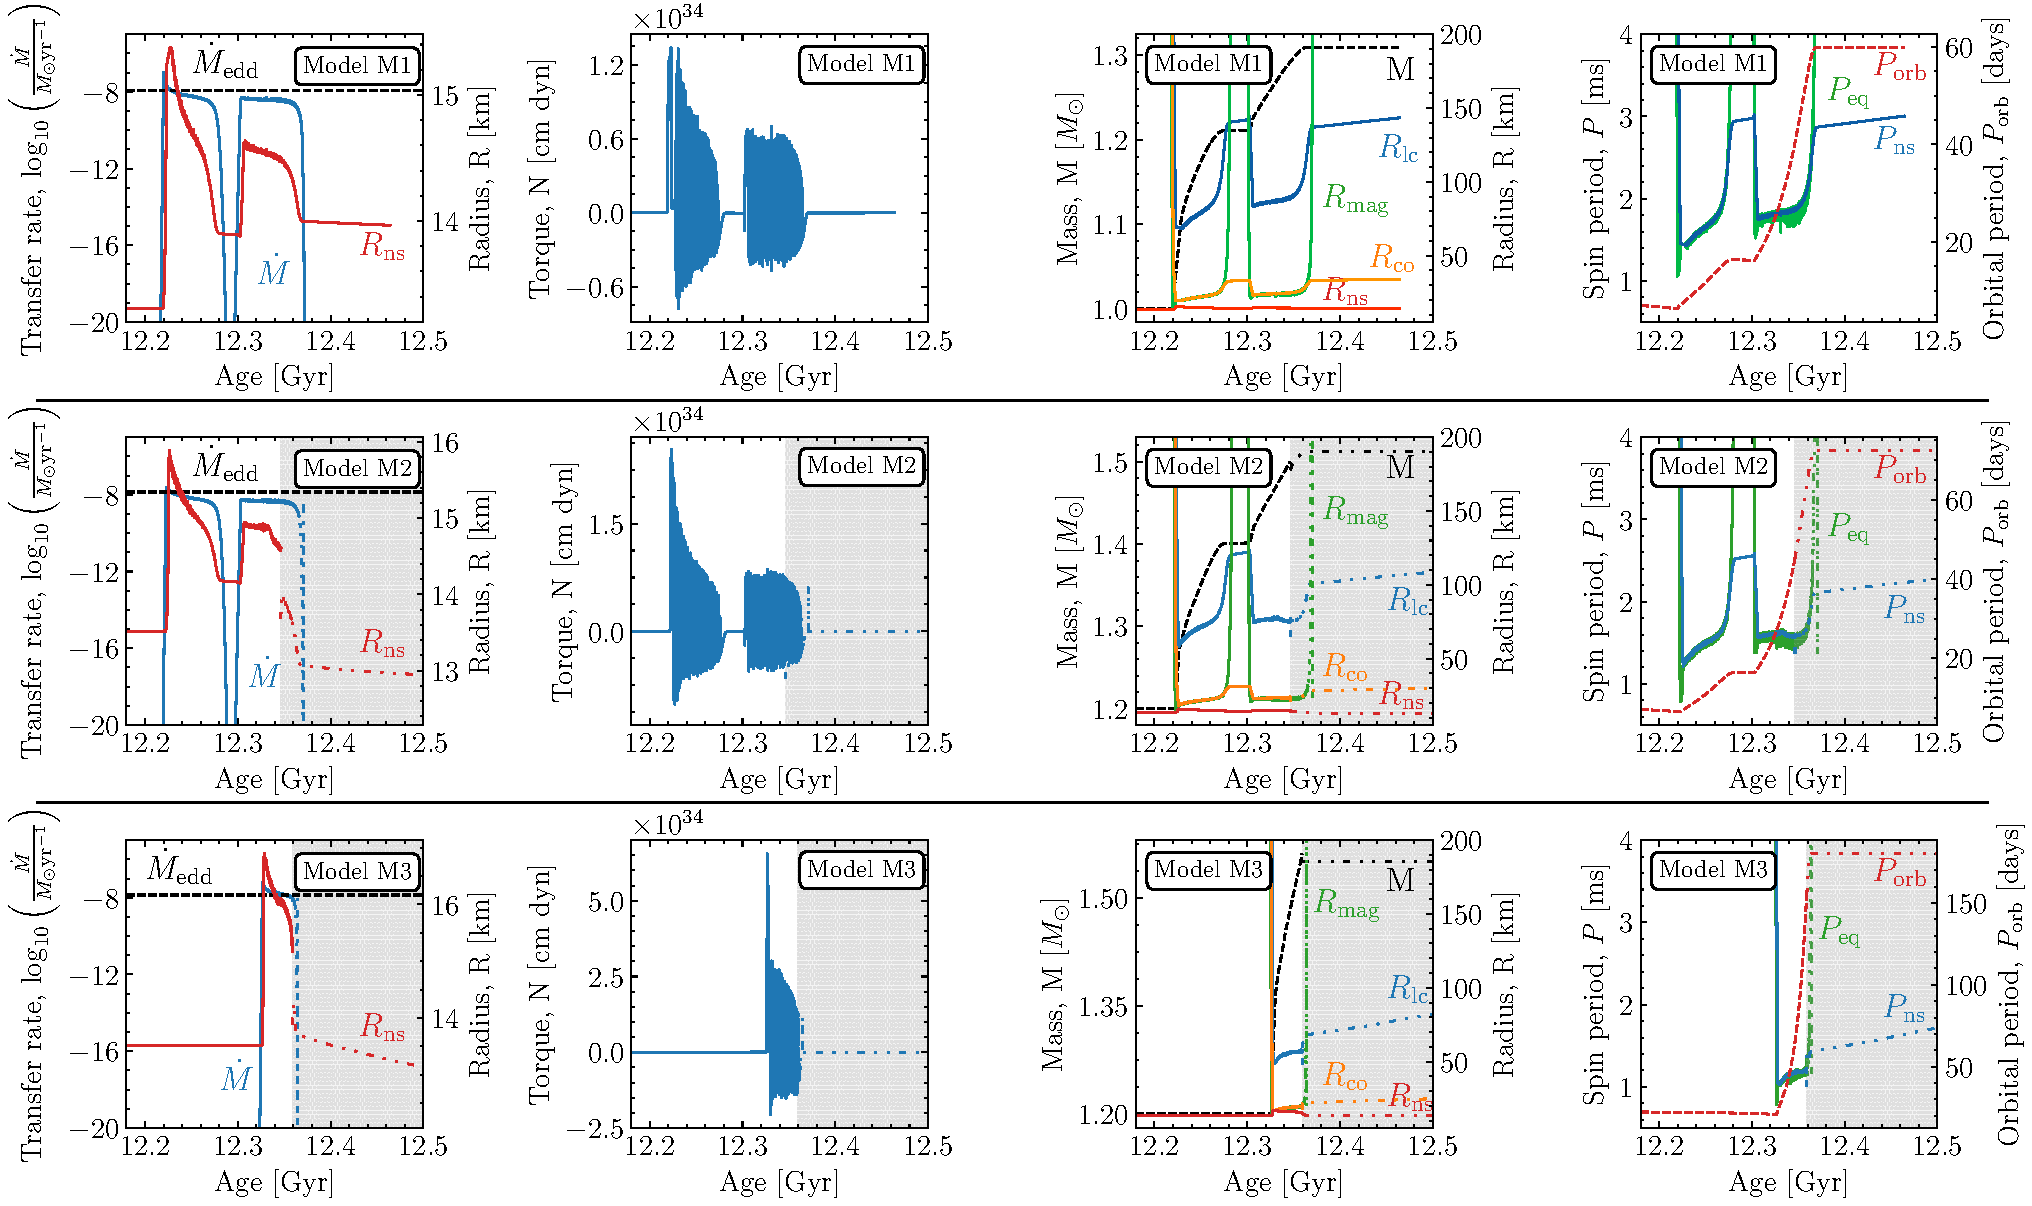
\includegraphics[width=\columnwidth,angle=0]{figures/chapter3/lmxb_grid.pdf}
            \caption{Summary of the evolution of the \textsc{m1} (top panel), \textsc{m2} (middle panel), and \textsc{m3} (bottom panel) models. The gray hashed region represents the posttransition evolution.}
            \label{fig:lmxb_grid}
        \end{figure*}   
        \end{landscape}
    




\end{document}